\documentclass[]{article}
\usepackage{lmodern}
\usepackage{setspace}
\setstretch{1}
\usepackage{amssymb,amsmath}
\usepackage{ifxetex,ifluatex}
\usepackage{fixltx2e} % provides \textsubscript
\ifnum 0\ifxetex 1\fi\ifluatex 1\fi=0 % if pdftex
  \usepackage[T1]{fontenc}
  \usepackage[utf8]{inputenc}
\else % if luatex or xelatex
  \ifxetex
    \usepackage{mathspec}
  \else
    \usepackage{fontspec}
  \fi
  \defaultfontfeatures{Ligatures=TeX,Scale=MatchLowercase}
\fi
% use upquote if available, for straight quotes in verbatim environments
\IfFileExists{upquote.sty}{\usepackage{upquote}}{}
% use microtype if available
\IfFileExists{microtype.sty}{%
\usepackage{microtype}
\UseMicrotypeSet[protrusion]{basicmath} % disable protrusion for tt fonts
}{}
\usepackage[margin=1in]{geometry}
\usepackage{hyperref}
\PassOptionsToPackage{usenames,dvipsnames}{color} % color is loaded by hyperref
\hypersetup{unicode=true,
            pdftitle={Component response rate variation underlies the stability of complex systems (revision notes)},
            pdfauthor={A. Bradley Duthie ( alexander.duthie@stir.ac.uk )},
            colorlinks=true,
            linkcolor=blue,
            citecolor=Blue,
            urlcolor=Blue,
            breaklinks=true}
\urlstyle{same}  % don't use monospace font for urls
\usepackage{graphicx,grffile}
\makeatletter
\def\maxwidth{\ifdim\Gin@nat@width>\linewidth\linewidth\else\Gin@nat@width\fi}
\def\maxheight{\ifdim\Gin@nat@height>\textheight\textheight\else\Gin@nat@height\fi}
\makeatother
% Scale images if necessary, so that they will not overflow the page
% margins by default, and it is still possible to overwrite the defaults
% using explicit options in \includegraphics[width, height, ...]{}
\setkeys{Gin}{width=\maxwidth,height=\maxheight,keepaspectratio}
\IfFileExists{parskip.sty}{%
\usepackage{parskip}
}{% else
\setlength{\parindent}{0pt}
\setlength{\parskip}{6pt plus 2pt minus 1pt}
}
\setlength{\emergencystretch}{3em}  % prevent overfull lines
\providecommand{\tightlist}{%
  \setlength{\itemsep}{0pt}\setlength{\parskip}{0pt}}
\setcounter{secnumdepth}{0}
% Redefines (sub)paragraphs to behave more like sections
\ifx\paragraph\undefined\else
\let\oldparagraph\paragraph
\renewcommand{\paragraph}[1]{\oldparagraph{#1}\mbox{}}
\fi
\ifx\subparagraph\undefined\else
\let\oldsubparagraph\subparagraph
\renewcommand{\subparagraph}[1]{\oldsubparagraph{#1}\mbox{}}
\fi

%%% Use protect on footnotes to avoid problems with footnotes in titles
\let\rmarkdownfootnote\footnote%
\def\footnote{\protect\rmarkdownfootnote}

%%% Change title format to be more compact
\usepackage{titling}

% Create subtitle command for use in maketitle
\providecommand{\subtitle}[1]{
  \posttitle{
    \begin{center}\large#1\end{center}
    }
}

\setlength{\droptitle}{-2em}

  \title{Component response rate variation underlies the stability of complex
systems (revision notes)}
    \pretitle{\vspace{\droptitle}\centering\huge}
  \posttitle{\par}
    \author{A. Bradley Duthie (
\href{mailto:alexander.duthie@stir.ac.uk}{\nolinkurl{alexander.duthie@stir.ac.uk}}
)}
    \preauthor{\centering\large\emph}
  \postauthor{\par}
      \predate{\centering\large\emph}
  \postdate{\par}
    \date{Biological and Environmental Sciences, University of Stirling, Stirling,
UK, FK9 4LA}

\usepackage{amsmath}
\usepackage{natbib}
\usepackage{lineno}
\usepackage[utf8]{inputenc}
\linenumbers
\bibliographystyle{amnatnat}

\begin{document}
\maketitle

\hypertarget{role-of-correlated-matrices-in-stabilisation}{%
\section{Role of correlated matrices in
stabilisation}\label{role-of-correlated-matrices-in-stabilisation}}

In complex systems represented by large random matrices, correlation
between matrix elements \(A_{ij}\) and \(A_{ji}\) affects the
distribution of eigenvalues and therefore local stability. As the
correlation between matrix elements (\(\rho\)) decreases, the eigenvalue
spectra changes such that more variation falls along the imaginary axis.
The figure panels below compare a random matrix in which \(\rho = 0\)
(left) to one in which \(\rho\) = -0.5. In both panels, complex systems
include \(S = 1000\) components, with diagonal elements of \(-1\) and
off-diagonal elements drawn from a normal distribution with a mean of
\(0\) and \(\sigma = 0.4\).

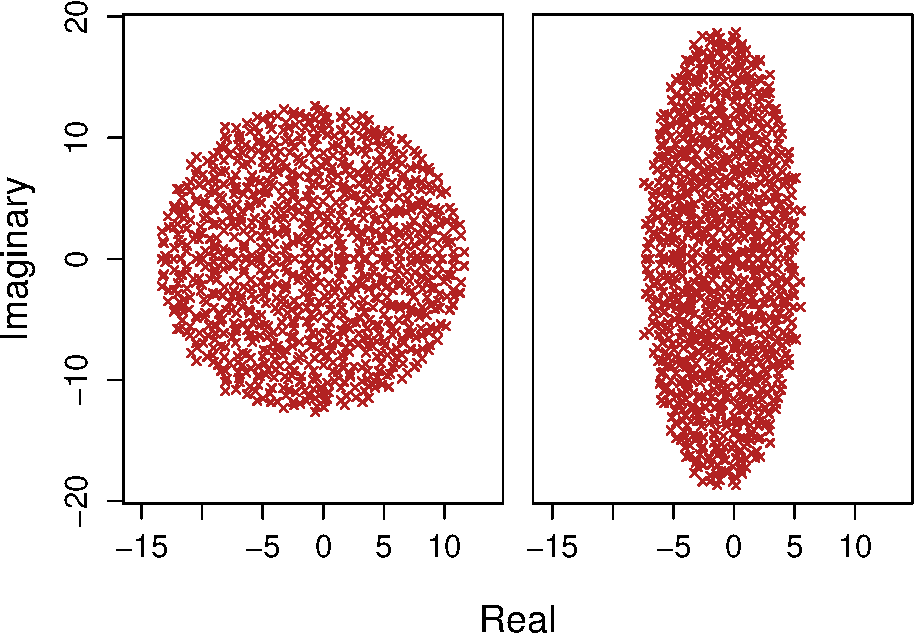
\includegraphics{revision_notes_files/figure-latex/unnamed-chunk-2-1.pdf}

Because of this effect of \(\rho\) on the eigenvalue spectra, decreasing
values of \(\rho\) will also tend to decrease the rightmost eigenvalue
of the matrix \(\textbf{A}\). This makes it more likely that the complex
system represented by \(\textbf{A}\) is locally stable, as stability
occurs when all real parts of eigenvalues are negative. Note that this
elongation along the imaginary axis is also characteristic of
predator-prey communities (in which, by definition \(A_{ij}\) and
\(A_{ji}\) have opposing signs). Also note that as \(\rho\) increases
such that \(\rho > 0\), the same elongation happens along the real axis,
making random complex systems less likely to be stable.

A simple numerical analysis illustrates the linear relationship between
\(\rho\) and the expected value of the real part of the leading
eigenvalue, \(\max(\Re(\lambda))\). Below, I have run 1000 simulations
across values of \(\rho\) from -0.9 to 0.9 for complex systems with
\(S = 25\) components. Error bars show 95\% bootstrapped confidence
intervals.

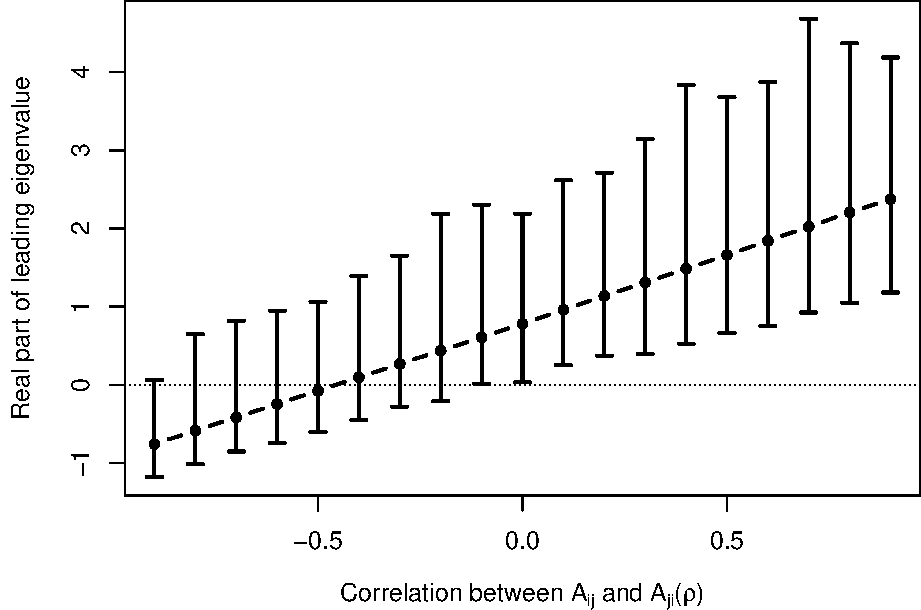
\includegraphics{revision_notes_files/figure-latex/unnamed-chunk-4-1.pdf}

In the main text, I demonstrated that when \(S\) is finite but system
complexity \(\sigma\sqrt{SC}\) is high (\(C\) defines the connectance of
\(\textbf{A}\), or the proportion of non-zero off-diagonal elements),
variation in component response rate \(\gamma\) often underlies system
stability. In other words, highly complex systems that are observed to
be stable would not be if we removed the variation in their component
response rates. Mathematically, this means that by multiplying
\(\textbf{A}\) by a diagonal matrix \(\gamma\) with variable elements,
the sign of \(\max(\Re(\lambda))\) is sometimes flipped from positive to
negative in these finite systems of high complexity. Interestingly, this
increase in stability given \(Var(\gamma) > 0\) is not necessarily
caused by \(\gamma\) decreasing \(\rho\). In fact, for \(S = 25\),
\(\sigma = 0.4\), and \(C = 1\), random complex systems that are
stabilised by \(\gamma\) typically have increased \(\rho\) values. Note
that for these parameter values, 1 million simulations found
\(\textbf{M} = \gamma \textbf{A}\) to be stable for 36 systems when all
\(\gamma_{i} = 1\), but 383 systems when
\(\gamma_{i} \sim \mathcal{U}(0, 2)\). Below shows the distribution of
the difference in \(\rho\) between systems with versus without
\(var(\gamma)\) for 1000 stabilised systems; that is,
\(\rho_{change} = \rho_{var(\gamma)} - \rho_{\gamma = 1}\).

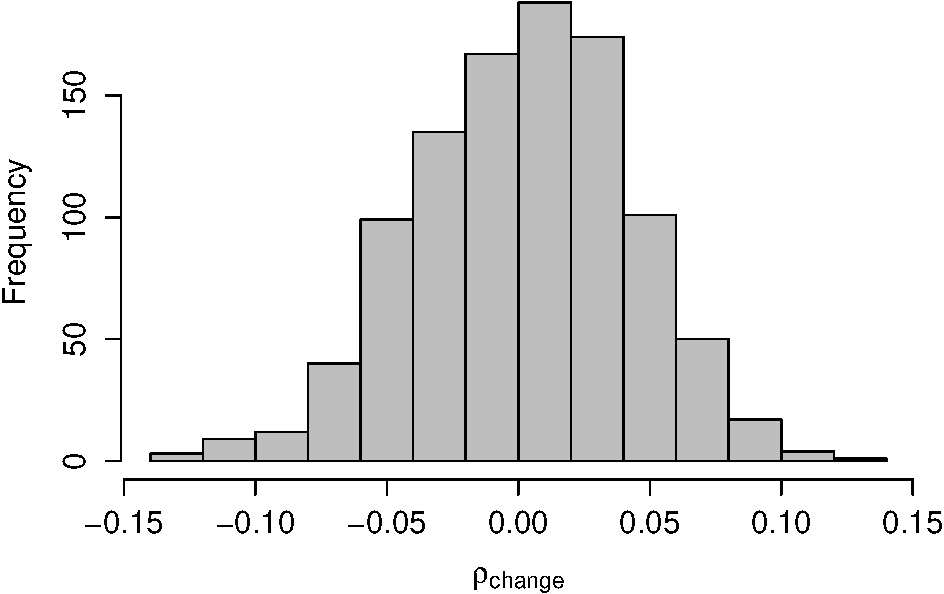
\includegraphics{revision_notes_files/figure-latex/unnamed-chunk-7-1.pdf}

When \(\textbf{A}\) was stabilised by \(Var(\gamma)\), the change in
\(\rho\) was normally distributed around 0.001414 (95\% CIs: -0.0011599,
0.0040885). Hence, decreasing the correlation between
\(\textbf{A}_{ij}\) and \(\textbf{A}_{ji}\) was not by itself the cause
of stability. For a clearer picture of the effect of \(\gamma\), it is
useful to show the relationship between \(\rho\) and
\(\max(\Re(\lambda))\) again as above with, but this time with how the
relationship changes given \(Var(\gamma)\).

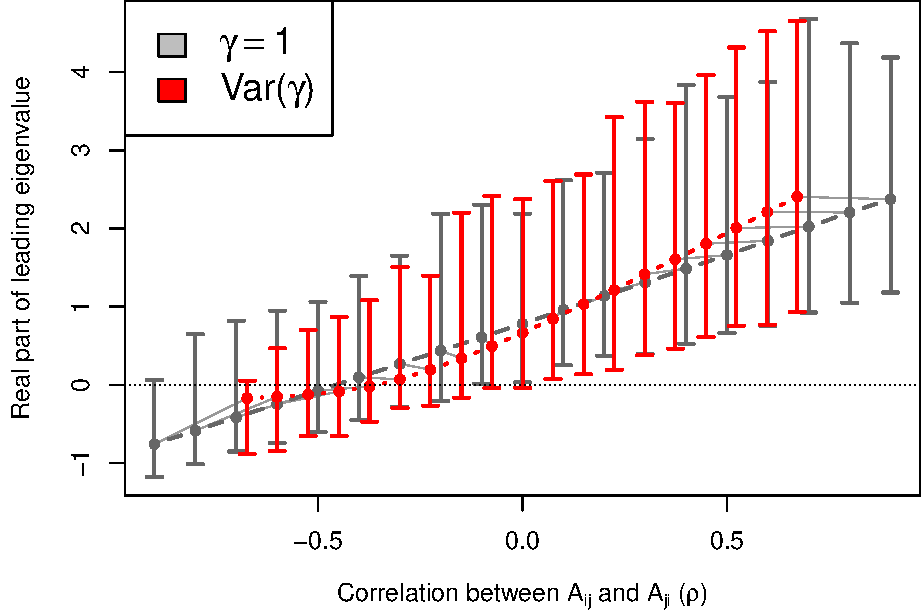
\includegraphics{revision_notes_files/figure-latex/unnamed-chunk-8-1.pdf}

Including \(Var(\gamma)\) introduces a nonlinear relationship between
\(\rho\) and \(\max(\Re(\lambda))\). Points along the x-axis are spaced
more closely together given \(Var(\gamma)\) because \(Var(\gamma)\)
tends to decrease the absolute magnitude of \(\rho\). Grey and red
points centred on \(\rho = 0\) represent the same simulations, before
(grey) and after (red) including \(Var(\gamma)\). Grey and red points to
the left and right show decreasing and increasing simulated \(\rho\)
values, respectively. Faint grey lines connect points for the same set
of simulations, and where the red point is lower than the black point,
the expected \(\max(\Re(\lambda))\) was lower given \(Var(\gamma)\).

The region of \(\rho\) values for \(\textbf{A}\) that would result in
increased stability given \(Var(\gamma)\) is highlighted with red
shading below.

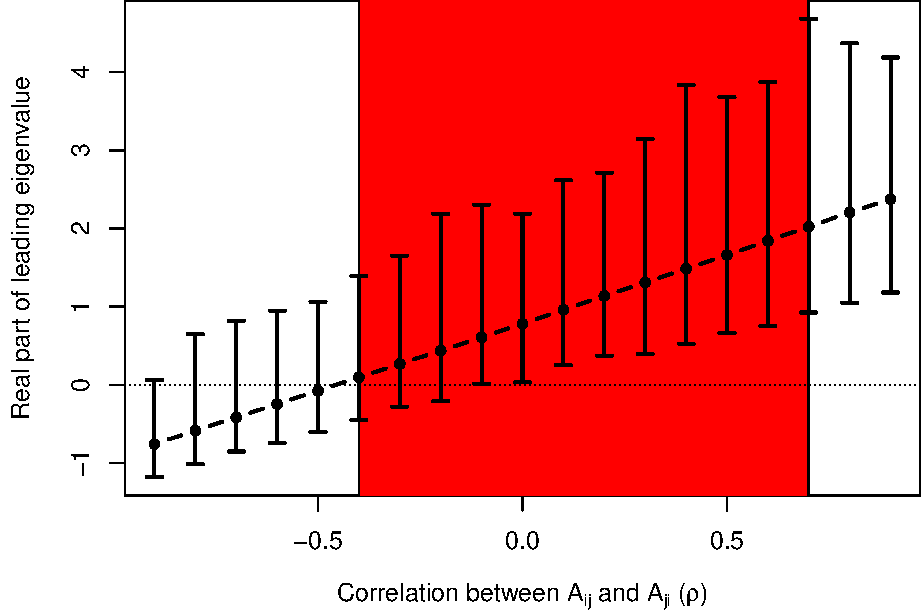
\includegraphics{revision_notes_files/figure-latex/unnamed-chunk-9-1.pdf}

In this red shaded region above, \(\max(\Re(\lambda))\) is decreased by
\(Var(\gamma)\). The shaded region encompasses values of \(\rho\)
between -0.4 and 0.7. But 1000 simulated \(\textbf{A}\) had values that
ranged between -0.240986 and 0.0704592, meaning that
\(\max(\Re(\lambda))\) was always expected to decrease given
\(Var(\gamma)\) even if \(Var(\gamma)\) caused \(\rho\) to increase.

The curvature of the relationship between \(\rho\) and
\(\max(\Re(\lambda))\) is consistent across different values of \(S\),
as shown below. Including \(\gamma\) always results in a concave upward
relationship between \(\rho\) and \(\max(\Re(\lambda))\).


\end{document}
